\section{Introduction}
This chapter will explore the state-of-the-art surrounding near field communication, gamification and persuasive technologies, along with some current solutions implemented by the industry.

It is anticipated that the main deliverable for this dissertation would be two Android mobile applications to facilitate the creation, deployment and management of a Loyalty Scheme. As such, we will need to discuss the pressing research, benefits and issues that encompass creation of `sticky' technologies on mobile platforms. 

\section{Near Field Communication (NFC)}
Near Field Communication (NFC) is an up-and-coming wireless technology that is currently being adopted in many contexts. Using this proximity-based standard, Two individuals can share data by placing NFC-enabled devices within a few inches of eachother.(see example in Figure 1.1). The standard was first established by Nokia, Philips and Sony in 2004 to define next generation radio frequency communications~\cite{nfcforum}.
\begin{figure}[H]
  \centering
    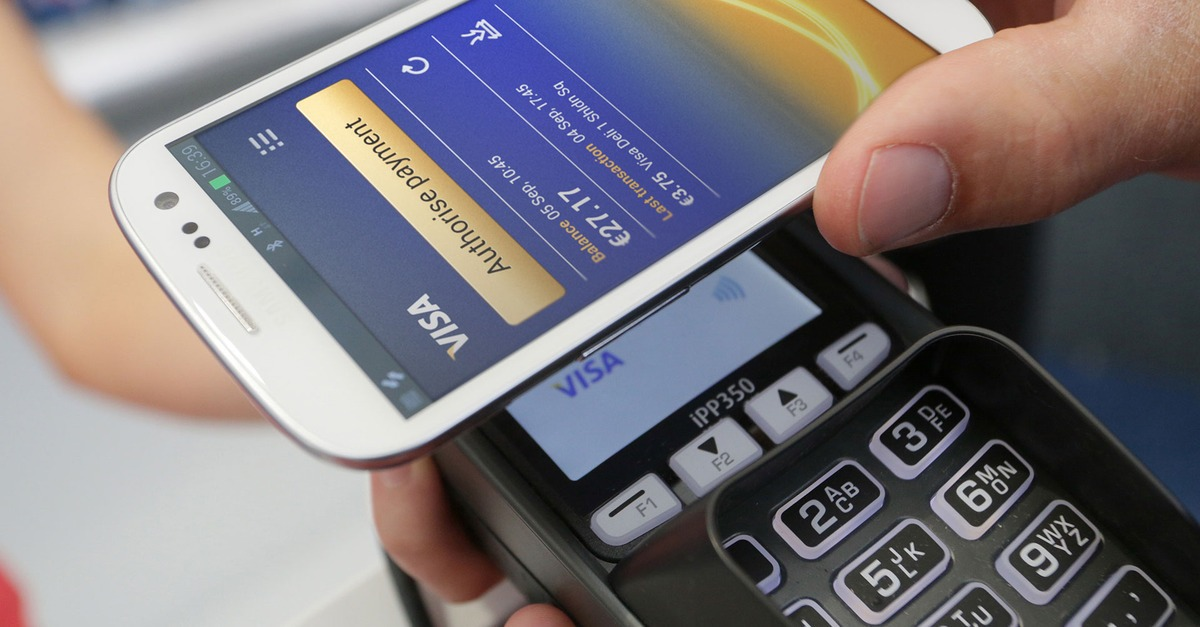
\includegraphics[width=1\textwidth]{img/visa-nfc-samsung.jpg}
      \caption{Using the smartphones NFC chip with a VISA application on a wireless card reader as a form of contactless payment}
\end{figure}

\subsection{Technical Fidelity of NFC}
NFC is a close relative to Radio Frequency Identification (RFID), using the 13.56 MHz radio frequencies under 424Kbit/s bandwidth~\cite{nfcloyal}; however it operates at a far shorter range (10cm versus 100m). As with RFID, there are two types of NFC devices - powered and unpowered. Powered devices surround themselves with an ultra-low power electrical field, inducing electric potential to other NFC devices within range; whereas unpowered devices (also known as ``tags''), rely on this electric potential from powered devices as a power source during the interaction.

NFC devices can adopt several different modes for different interactions~\cite{ventata}

\paragraph{Tag Reading/Writing}
A powered NFC device in this mode can read and write information stored in tags. Websites,  contacts and telephone numbers are commonly encoded in this manner. Upon reading the tag, it is the software's responsibility to act on the data in an appropriate manner~\cite{ecosystem}

\paragraph{Host Card Emulation}
NFC chips can be placed into Card Emulation mode in such a way (ISO 14443)~\cite{iso14443} that a card reader classifies it in the same manner as a smartcard. NFC devices can keep different cards in storage and switch between emulating them as required.~\cite{ecosystem}

\paragraph{Peer-to-Peer}
Two powered NFC devices can bidirectionally share information between each other - for instance Bluetooth pairing information.~\cite{ecosystem}. In the case of a business environment, authentication can take place between two devices in the same bidirectional manner~\cite{iso18092} as a form of `secure log-in'.

\subsection{NFC as an Interaction}
%quick pairing
%people tap eventhough there is no need
lorem ipsum
\clearpage{}
\subsection{Applications of NFC}
Wireless communication technologies such as NFC have been around for some time. Many electrical devices with the capacity to communicate already use Wi-Fi, Infrared or Bluetooth; eventually these technologies make their way into modern smartphones and other domestic devices. Due to the openness of the NFC standard, there are a wide plethora of implementations facilitated by the technology:
\paragraph{\textbullet~Contactless Payment/Mobile Wallet}
Starting from 2005, banks began integrating contactless chips inside debit/cards for payments under 20 USD/GBP (provided that the card reader supported contactless). From 2011, several large players such as Google, Apple and Paypal have developed mobile wallet applications, with Google and Apple primarily supporting NFC. Contactless cards too rely on the (ISO 14443)~\cite{iso14443} smartcard standard, complementing the previously discussed host card emulation, allowing an NFC chip to emulate an identical smartcard. Whereas, contactless debit and credit cards are prevalent, Google Wallet and Apple Pay are not available outside of the US Market, reasonings being ill-documented.
\paragraph{\textbullet~Ticketing}
Contactless ticketing has been available for a while, the Oyster card\cite{oystercosts} being an iconic example; nonetheless it has the issue of being a proprietary, locked down technology. In 2014, contactless cards were enabled within the system. Some argue that the goal of removing cash-payments was a driving factor of the acceptance of contactless ticketing~\cite{oystercosts}. Moreover, Host Card Emulation infers that mobile wallet applications would also be able to take advantage of these readers.
\paragraph{\textbullet~Gaming}
Game designers have always looked for ways to make video games more engaging. There are two methods in which they can implement NFC within their games, with the intent to make \textbf{Pervasive Games}. Such games expanding the play space into the player's ordinary social life~\cite{montola2005exploring}. Firstly, they may may use NFC to enrich collaboration and sociability. As an example, a study was done with two identical games, one with NFC and the other without\cite{wolbert2013evaluating}. Experiments were ran with two groups of individuals and findings showed a sharp increase in positive experience for NFC over touchscreen~\cite{wolbert2013evaluating} 

The second and more recent way NFC can be implemented in video games is through physical-digital mappings. The \emph{Wii U}~\cite{nintendo} video game console contains an NFC chip in the controller, allowing users to use NFC enabled figurines on the controller. The result of tapping these devices together makes figurines appear within the console as in-game characters. 

\paragraph{\textbullet~Loyalty Schemes}
Loyalty using NFC is a topic that is still being explored by industry. As such, there are some different and creative implementations available. The original NFC Loyalty solutions came in the form of staff/store cards; however with the advent of NFC in mobile phones, pervasive solutions have been implemented such as \emph{Orange EAT}~\cite{orangeEat}.  In this scheme, consumers can tap specific NFC posters and tags in order to gain free rewards in the form of food and drink~\cite{orange}. Unfortuantely this promotion was unsuccessful as at the time only 200,000 customers had an NFC enabled device on Orange (less than 1\% of the total customer base)~\cite{orange}. There are several other prototype solutions available; nonetheless they were not properly adopted as NFC was not available on enough phones.
\clearpage{}
\subsection{NFC in Phones}
NFC functionality in phones is actually not a new concept; phones with NFC chips have been around since 2006, but the adoption of NFC with manufacturers did not get popular until 2010 when a set of peer-peer standards were released to transfer useful information (contacts, URLs and bluetooth)~\cite{iso18092}. Since then, popularity took off, with IHS\footnote{IHS inc is a data and critical information provider for the technology industry} predicting that 939 million NFC enabled handsets would be shipped in 2018 (Fig. \ref{fig:smartphoneshipments})~\cite{IHSchart}.
\begin{figure}[H]
  \centering
    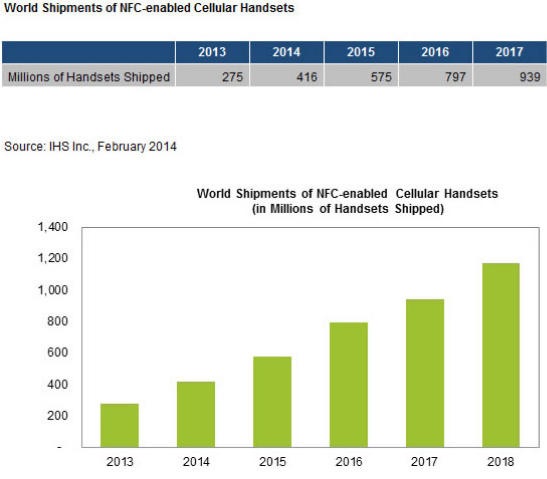
\includegraphics[width=0.8\textwidth]{img/smartphoneNFC.png}
      \caption{A chart depicting the predictions of mobile phones shipments that have NFC built-in}
       \label{fig:smartphoneshipments}
\end{figure}

Interestingly, of all the applications mentioned in the above section, \textbf{all} of them have been implemented both with and without mobile phones. The advantage of using the mobile phone is that it has the capability to consolidate a potentially infinite amount of NFC cards, tags etc into just one chip.

Software support for NFC is something that must be accompanied with hardware. Android and Symbian implemented software support in 2011, Microsoft in 2012 and Apple in 2014. The fact that these implementations are very recent can be attributed to the rising popularity of NFC. 

\subsection{Areas of Research}
In 2010 a survey was done of academic papers surrounding NFC \cite{nfctable}. The authors gathered a total of 74 research papers and used content-oriented classification~\cite{ngai2008rfid} in order to split up NFC papers into four categories: NFC Theory, NFC Applications, NFC Infrastructure and NFC Ecosystem. The results of their findings are shown in table \ref{table:nfcresearch}.
\begin{table}[H]
\resizebox{\textwidth}{!}} \\ \midrule
\multicolumn{1}{|l|}{\begin{tabular}[c]{@{}l@{}}\textbf{NFC Applications and Services}\\ Reader-Writer Mode Applications\\ Host Card Emulation Applications\\ Peer-to-Peer Applications\end{tabular}} & \multicolumn{1}{l|}{Discussing or developing different implementations of NFC applications and services based of NFC modes} & \multicolumn{1}{c|}{30} & \multicolumn{1}{c|}{\begin{tabular}[c]{@{}c@{}}\textbf{40.5}\%\\ 25.7\%\\ 13.5\%\\ 1.35\%\end{tabular}} \\ \midrule
\multicolumn{1}{|l|}{\textbf{NFC Infrastructure}} & \multicolumn{1}{l|}{Types of NFC technologies and their applications in the real world, also security and privacy} & \multicolumn{1}{c|}{22} & \multicolumn{1}{c|}{\textbf{29.7\%}} \\ \midrule
\multicolumn{1}{|l|}{\textbf{NFC Ecosystem}} & \multicolumn{1}{l|}{frameworks for businesses that want to integrate NFC culture \& models and strategies into their processes} & \multicolumn{1}{c|}{7} & \multicolumn{1}{c|}{\textbf{9.5\%}} \\ \bottomrule
\end{tabular}
}
\caption{Table showing the primary categories of NFC research}
\label{table:nfcresearch}
\end{table}

It can be observed that a huge proportion of NFC literature (40\%) at the time was heavily focused on developing prototype applications and services. However, the specific types of applications were primarily `Reader-Writer' mode as this was just before the introduction of NFC peer-to-peer standards.

The research identified that there was a gap in researching the development of NFC principles and theories or how to integrate such solutions into business models. As a result, we can argue that this business-orientated business gap was a factor for the slow adoption of NFC.
\subsection{Limitations of NFC}
The key limiting factor of NFC for the longest time was the slow adoption rate by businesses and manufacturers. Contactless payment, the predominate form of NFC interaction depended on specific NFC card readers to enable contactless functionality; furthermore we cannot underestimate the amount of effort it takes to introduce a new billing option to a country.

Analytics also show that NFC implementations are very fragmented with no apparent standard protocols~\cite{fragmentednfc}. This can be attributed to two reasons: the openness of the NFC platform encouraging different implementations and businesses wanting their own implementation for their own needs. For instance, in the example of loyalty schemes, each business might have a separate loyalty application which the customer needs to download and setup. These applications allow businesses to perform their own tracking and branding.
%very short range of NFC makes it difficult to eavesdrop on
\subsection{QR and NFC}
%%%%%%%%%%%%%%%%%%%%%%%%%%%%%%%%%%%%%%%%%%%%%%%%%%%%%%%%%%%%%%%%%%%%%%%%%%%%%%%%%%%%%%%%%%%
%                                 GAMIFICATION SECTION
%%%%%%%%%%%%%%%%%%%%%%%%%%%%%%%%%%%%%%%%%%%%%%%%%%%%%%%%%%%%%%%%%%%%%%%%%%%%%%%%%%%%%%%%%%%
%About 20 percent of phones worldwide might have NFC capabilities by 2014 [source: Juniper].
\clearpage{}
\section{Gamification}
Over the years, a keen topic of research within Human Computer Interaction is that of user engagement. There are several different design models that afford this goal. One recent and popular example being gamification. 

Gamification can be best described as
\begin{quotation}
\noindent
``An informal umbrella term for the use of video game elements in non-gaming systems to improve user experience (UX) and user engagement.''~\cite[p.~2425]{Deterding:2011:GUG:1979742.1979575}
 \end{quotation}

%talk about user engagement stuff/ studies
The need for gamification comes from the modern zeitgeist of the digital world, a world of engagement. Comparing the current opportunities for entertainment (i.e. video games, social media, the internet) to those from fifty years ago, provide users with much more choice. Furthermore, users are no longer registering traditional advertising in the same way they did fifty years ago. A study done with university students using eye-tracking technology with \emph{Facebook} shows that students perceive less than a quarter of the site's adverts~\cite{barreto2013users}. Experimenters concluded that this was due to users scrolling the timeline too quickly and learning where advertisements appear, therefore ignoring those areas. 

By harnessing the power of play, designers can apply motivational affordances to improve user engagement. Gamification techniques are predicted as the future of marketing~\cite{ventata}, with Gartner\footnote{Gartner is an IT research and advisory business} stating that 50\% of companies with innovation processes will incorporate gamification by 2015~\cite{gartner50}.

\subsection{History}
The principles of ``turning things into games'' are actually not new. They have long been employed by parents and teachers to make activities seem more enticing to children; however applying game-like aspects to a business environment was only formally introduced in the 80's~\cite{coonradt1985game}. The word \emph{Gamification} was coined in 2002 by Nick Pelling, an early computer games programmer that wanted to apply game-mechanics to different contexts~\cite{marczewskigamification}. Recently, gamification has become a buzzword amongst modern system designers. The rise in popularity can be shown in a Google Trends search (Fig. \ref{fig:gamificationpopularity}). This boom can be attributed to soaring video game popularity and cheap enabling technologies found in modern domestic appliances (i.e GPS, Internet Access, Bluetooth etc.)~\cite{Deterding:2012:GDM:2212877.2212883}

\begin{figure}[H]
  \centering
    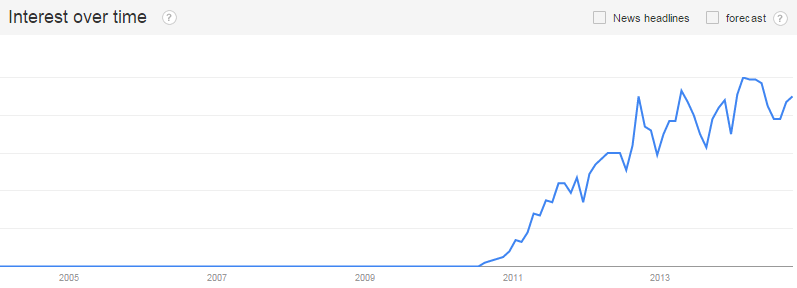
\includegraphics[width=1\textwidth]{img/gamification.png}
      \caption{Google Trends graph depicting the search popularity of the term \textbf{Gamification} over the years}
      \label{fig:gamificationpopularity}
\end{figure}


The use of gamification has also shifted over the years. Many reseachers~\cite{deterding2014ambiguity}\cite{park2014study} consider Charles Coonradt as pioneer in the field of gamification. In his acclaimed book \emph{The Game Of Work}~\cite{coonradt1985game}, Coonradt introduces ``game-like concepts'' inspired from sports as a means to increase employee productivity, satisfaction and motivation~\cite{coonradt1985game}. On the other hand, gamification in the digital age takes inspiration from video games to to improve user experience, engagement and loyalty.~\cite{ventata}

It can be argued that the two inspirations (sports vs. video games) present us with different flavours of gamification. Games of sport entail clear goals, instantaneous feedback, and the concept of striving to be better. Video games aim to keep players playing by providing psychological rewards such as achievements, unlocks and ability to compare their skill with their friends. Even though these two methods of gamification have some differences, their main shared trait lies in the way they play on our natural instinct of socialisation and competition. ~\cite{grove2011gamification}

\subsection{Gamification and Mobile Technologies}
Although elements of gamification can be found in a variety of systems, mobile technologies have seen biggest boom in gamified systems. As mentioned earlier, a major contributer to this boom is the prevalence of cheap enabling technologies such as bluetooth, and GPS - all of which can be found on a modern smartphone. In 2009, Foursquare was one of the first successful gamified mobile applications; allowing users to ``check-in'', collect badges and receive recommendations on where to go next~\cite{zichermann2011gamification}. Five years later, Gartner predict that 70\% of the top 2000 companies would have a gamified application by the end of 2014.~\cite{gartner70}

\subsection{Areas of Research}
Areas of research of gamifcation using certain elements...
\clearpage{}
\subsection{Critiques of Gamification}
The application of gamification practises to digital applications is prevalent amongst business applications~\cite{gartner70}, nonetheless these practises have attracted criticisms. One view adopted by the video games industry is that gamification mistakenly portrays ``game-like'' properties, such as levels and scores as part of human behavioural complexity.~\cite{bogost2011gamification}. Moreover, there are negative ``exploitative'' connotations (discussed later) to word gamification in the business world; therefore businesses generally prefer the term ``motivational design'' instead. 

The concept of creating ``sticky'' systems via gamification techniques can also present us with systems that affect user behaviour negatively. The McDonalds Monopoly sweep-stake is a well known example of this phenomenon. The promotion involves the collection of monopoly stickers containing prizes from purchasing certain food and drink (more stickers with larger meals). Paxman et al~\cite{mcdonalds} introduce examples where consumers change their purchasing habits in order to maximise the number of stickers they receive, linking these changes to childhood obesity~\cite{mcdonalds}. Several theories of motivation exist explaining these behaviours; however Zichermann~\cite{zichermann2011gamification} considers motivational factors as unruly, yet admits ``once you start giving someone a reward, you have to keep [them] in that reward loop forever''~\cite[p.~27]{zichermann2011gamification}.

%%%%%%%%%%%%%%%%%%%%%%%%%%%%%%%%%%%%%%%%%%%%%%%%%%%%%%%%%%%%%%%%%%%%%%%%%%%%%%%%%%%%%%%%%%%
%                                PURSUASIVE SYSTEMS
%%%%%%%%%%%%%%%%%%%%%%%%%%%%%%%%%%%%%%%%%%%%%%%%%%%%%%%%%%%%%%%%%%%%%%%%%%%%%%%%%%%%%%%%%%%
\section{Persuasive Technologies/Captology}
Capturing the attention of an person for the purposes of persuading them is a problem that sympathises with many. Businessmen, politicians and teachers alike are examples of such professions - more specifically professions where persuasion is an integral factor of their success. There exist a plethora of methods to achieve this, for instance salesman study marketing, politicians study public speaking, whilst those in the realm of technology study captology (the art of persuasive technologies).

We can define `persuasive technologies' as:
\begin{quotation}
\noindent
Solutions which are designed with a purpose to change attitudes or behaviours via persuasion and social influence, but not through coercion~\cite{fogg}[p.10]
\end{quotation}

Fogg, considered by many~\cite{fogg1}\cite{fogg2} as a pioneer in the research of captology, identifies the art as an intersection between technology and persuasion (Fig. \ref{fig:captologyVenn}). 

\begin{figure}[H]
  \centering
    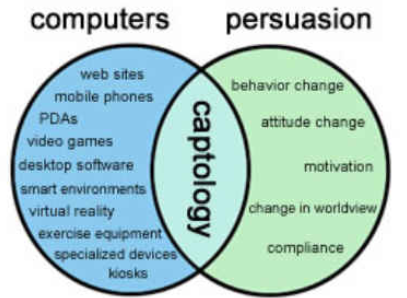
\includegraphics[width=0.5\textwidth]{img/captology-figure-3.png}
      \caption{A Venn diagram showing the intersection of persuasion and technology - Captology}
      \label{fig:captologyVenn}
\end{figure}

\subsection{Types Of Motivation}
It is also helpful to mention the types of motivations which affect people to do activities. Literature indicate that there are three main types of motivators that drive people to behave in a certain way, Deci and Ryan~\cite{motivationtypes} define them as:
\begin{quotation}
\noindent
\textbf{Extrinsic Motivation}~ Incentives where motives to enact the task are not related necessarily to that specific behaviour - \textit{i.e. Completionism}

Extrinsic motivation takes the form of leveraging the human Psyche. For instance, the example of a progress bar persuades the user to bring it up to 100\%. The user may not be specifically motivated to perform the task, but they are motivated to complete the progress bar.
\end{quotation}
\begin{quotation}
\noindent
\textbf{Intrinsic Motivation}~ The act of making the intended behaviour so pleasurable that it becomes an end in itself - \textit{i.e. Gamification}

The philosophy of this motivator is to persuade the user to engage with the activity in a way that they enjoy. Gamification exists within this realm of motivation, making activities more enticing to users.
\end{quotation}
\begin{quotation}
\noindent
\textbf{Tangible Motivation}~ External Incentives driving the motivations - \textit{i.e.Rewards/Money}

These motivators usually offer some sort of reward such as money to entice the user to perform an action. Although only considered as short-term, it is useful at incentivising one-off activities that are difficult to make engaging, for example surveys. 
\end{quotation}

Persuasive technologies afford the use of any combination of these to develop systems. We discuss an example in Sec. \ref{sec:piano}

\subsection{Fogg's Taxonomy}
Fogg characterises each persuasive technology by \emph{functional roles}: tools, media or social actors.~\cite{fogg1998persuasive}, of which technologies can identify as one or several of these categories. The proposed triad is designed to model the way in which users see and react to the following:

\paragraph{Tools}
These technologies are designed to make people's jobs easier\cite{fogg}. For example a wizard or an Out of Box Experience (OOBE) can give users direction regarding the completion of a specific or complex user task.
\paragraph{Media}
Media-centric technologies are designed to provide users a platform to create experiences that develop, teach or enforce a behaviour. These can come in the form of games, interactive systems or stories;  the best examples however are simulations. Simulations place the users in a specific environment where they must interact with rules of the system in order to hone a required set of behaviours; such behaviours can be for the purposes of testing or real-life skills. 
\paragraph{Social Actors}
With the introduction of social actors, computer systems can now influence users using social cues. Actors can be persuasive by giving a human face to positive feedback, modeling an inded behavior or provide moral support to the user~\cite{fogg}. The \emph{Microsoft Paperclip} is a famous example of a social actor to teach users how to use Microsoft Office. Research in this area is constantly developing as it's difficult to build `human' characters without entering ``uncanny valley''.
 
%A social actor can be persuasive byreddit.com
% Rewarding people with positive
%feedback
% Modeling a target behavior or
%attitude
% Providing social support

\subsection{Persuasive Technologies Through Gamification}
\label{sec:piano}
Persuasive Technology is a broad term. As such, it can be argued that gamification exists within the realm of captlogy; nonetheless there exists the key differentiators of scope, more specifically - gamification is not necessarily linked to technology (although `gamified' technologies are generally more common).
%gamification just makes something more enticing , whereas captology

A well known case study of implementing persuasive technologies using gamification are The Piano Stairs (Fig. \ref{ref:pianostaircase})~\cite{tieben2011curiosity}. In this example, tiles and speakers in the configuration of a piano were installed next to an escalator, each stair playing a specific note on the piano when stepped on. The purpose of this experiment was to get more commuters to take the `healthier' stairs rather than the escalator. Results showed that people were taking the stairs frequently and in more `musical ways', with some musicians attempting to play songs using them. There was however another factor that encouraged people to take the stairs: curiosity~\cite{tieben2011curiosity}. The staircase is so out of place that people are curious and thus want to explore and engage with the technology.

\begin{figure}[H]
  \centering
    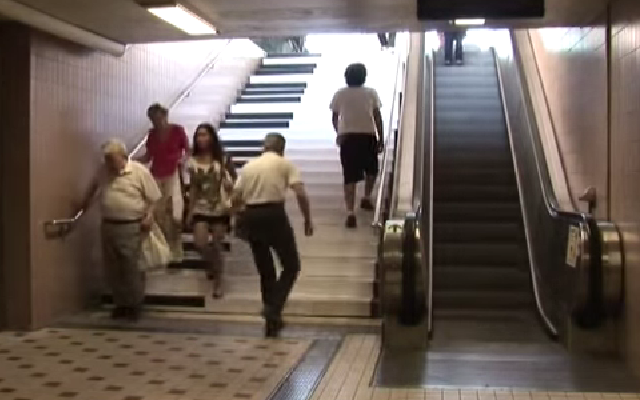
\includegraphics[width=0.7\textwidth]{img/pianotiles.png}
      \caption{The piano tiles staircase}
      \label{ref:pianostaircase}
\end{figure}

Applying the concept of Fogg's taxonomy and motivator types, this innovation is an example of a media-oriented technology, fueled by intrinsic motivation - making the act of going up the stairs more enjoyable. Although empirical evidence on users after taking the stairs was not tracked, it would be interesting to see whether these stairs impacted people's choice of taking other stairs in the long run. 

%%%%%%%%%%%%%%%%%%%%%%%%%%%%%%%%%%%%%%%%%%%%%%%%%%%%%%%%%%%%%%%%%%%%%%%%%%%%%%%%%%%%%%%%%%%
%                                     SOLUTIONS
%%%%%%%%%%%%%%%%%%%%%%%%%%%%%%%%%%%%%%%%%%%%%%%%%%%%%%%%%%%%%%%%%%%%%%%%%%%%%%%%%%%%%%%%%%%
\clearpage{}
\section{Survey of Technologies}
We now turn our focus to the developed solutions. These technologies were chosen as they use a combination of NFC, gamification or persuasive technologies. The first group will contain implementations dedicated to a certain business; whereas the second will look at more generic applications. The chosen solutions were only those where \textbf{Loyalty} was the core function of the technology, `ecosystem-based' combined solutions were not considered.

In order to summarize these technologies later, each of the following should answer these questions:
\begin{itemize}
  \item How does the user interact between the real world and the applications (what pervasive elements does the application possess)?
  \item What elements of gamification exist?
    \item In what ways are multiple loyalty schemes presented? %levelling up - multiple schemes 
  \item Are there any subtle persuasion techniques employed?
\end{itemize}


\begin{figure}[H]
  \centering
    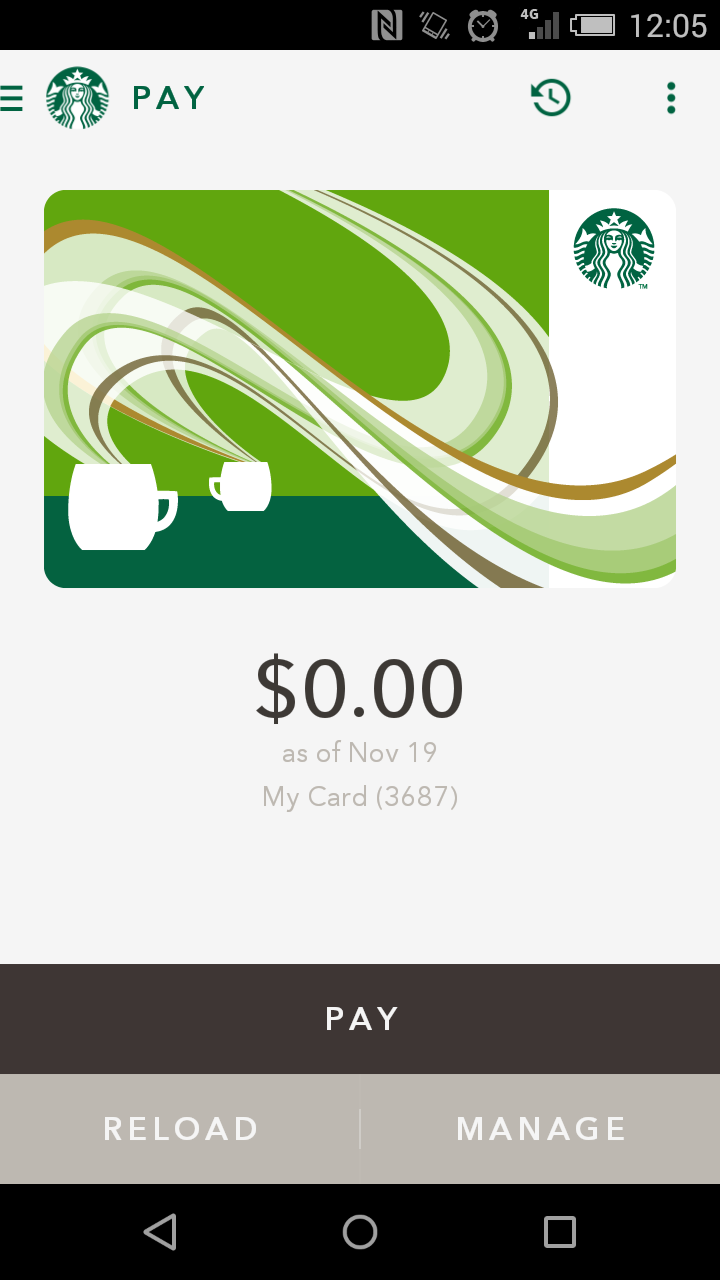
\includegraphics[width=0.24\textwidth]{img/starbucks.png}
    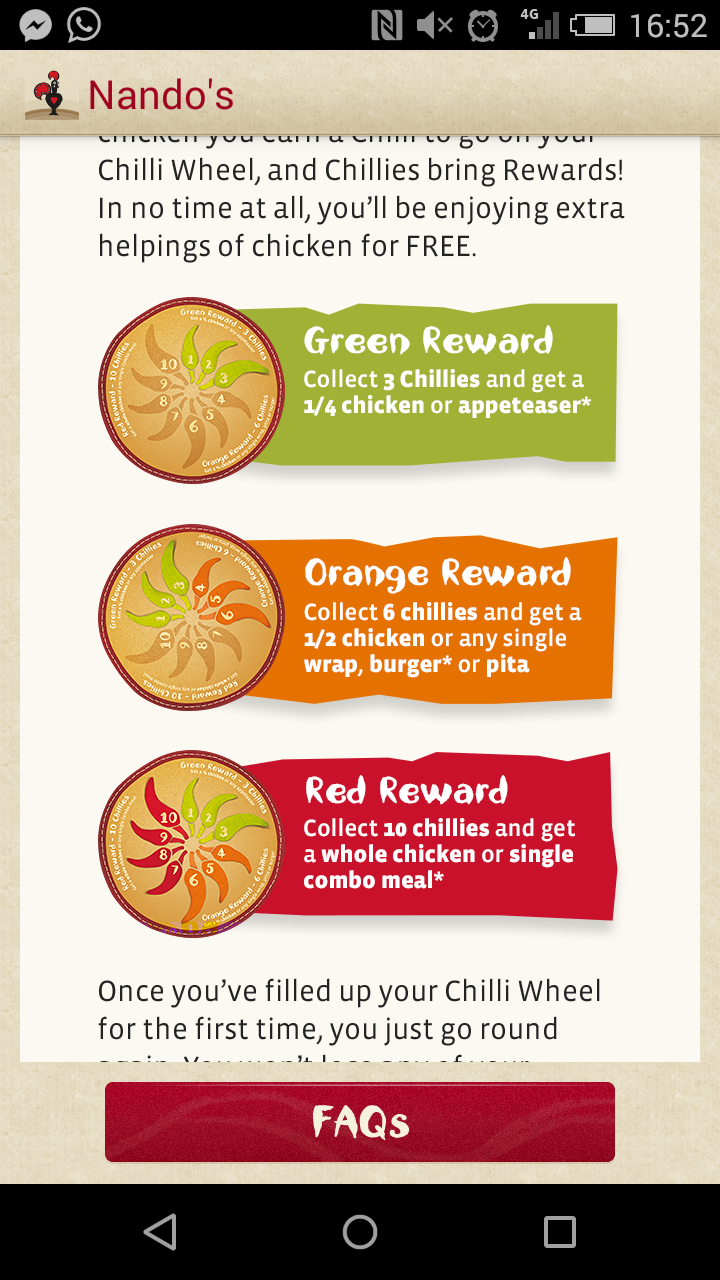
\includegraphics[width=0.24\textwidth]{img/nandos.png}
    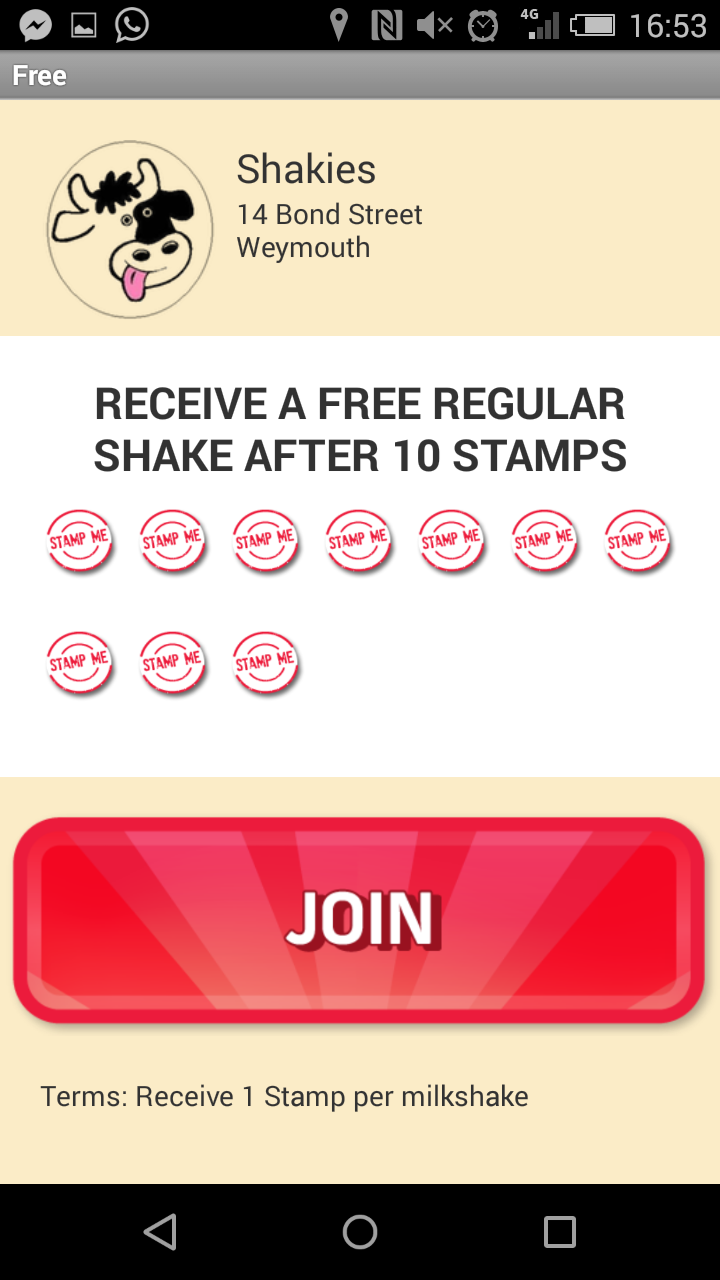
\includegraphics[width=0.24\textwidth]{img/tagmate.png}
    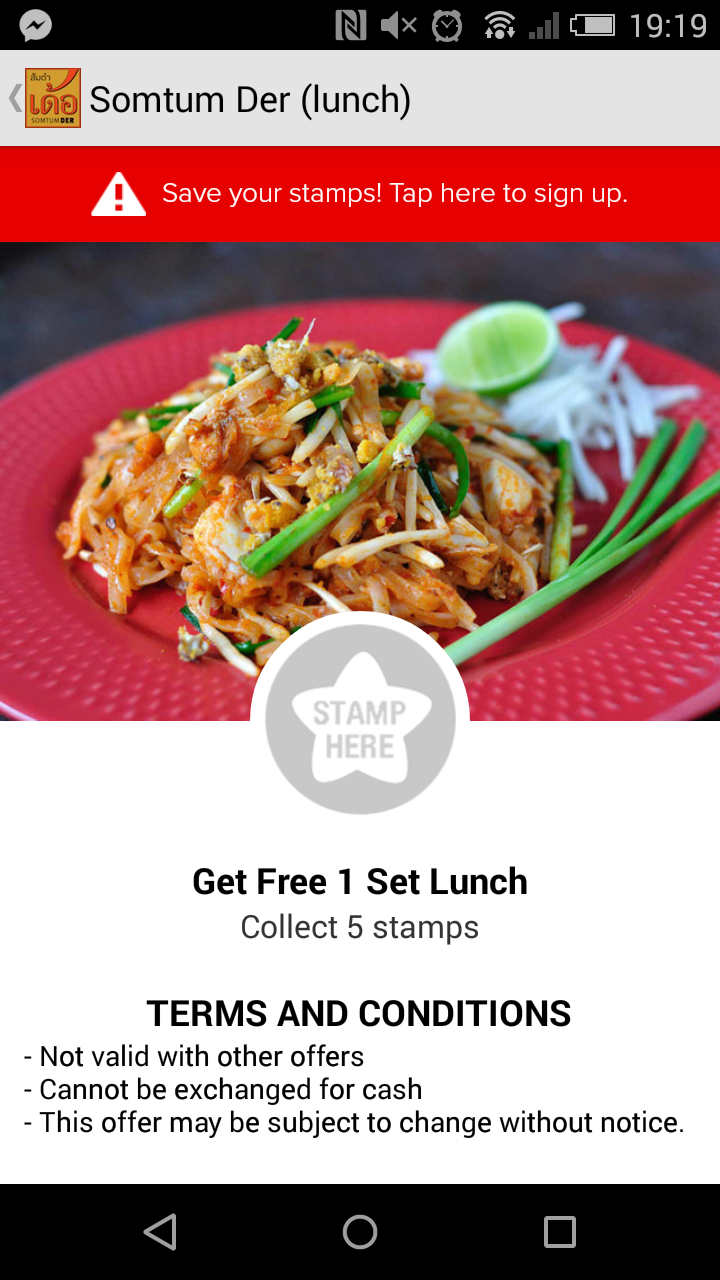
\includegraphics[width=0.24\textwidth]{img/stamp.png}
      \caption{The technologies to be analysed: (a) Starbucks (b) Nandos (c) StampMe (d) Stamp}
\end{figure}

\newpage
\subsection{Starbucks Mobile Application}
\textbf{Overview}
The Starbucks mobile application is designed as a digital-companion to the standard plastic loyalty card they provide. The application allows user's to either have a digital-only card or transition their physical cards onto the app, allowing customers to view, top up and pay with their balance.

\textbf{What are the pervasive elements?}
Aliased Card Using BQ barcode that is scanned by a barista.

\textbf{What elements of Gamification exist?}
Collect Stars with each purchase, free drink on 15, upgrade to gold member upon collecting 50 stars.


\textbf{In what ways are multiple loyalty schemes presented?}
The user can have up to 10 Starbucks cards but only claim free drinks with their stars.

\textbf{Are there any subtle persuasion techniques employed?}
Extrinsic Motivation of filling a cup, personalise your card.
%personalise card

\subsection{Nandos Mobile Application}
\textbf{Overview}
As with Starbucks, the Nandos' mobile application works in a very similar manner to the starbucks card. It allows users to register their current physical card; however this app is purely as a companion, informing users of the status of their loyalty points in the card.

\textbf{What are the pervasive elements?} There are no pervasive methods. The user must have and use a Nandos Card.

\textbf{What elements of Gamification exist?}
No elements of gamification are used.

\textbf{In what ways are multiple loyalty schemes presented?}
Loyalty schemes are presented as a progressive stampcard. Rewards of increasing value are granted upon reaching certain amounts of chillis

\textbf{Are there any subtle persuasion techniques employed?}
When a users connects their card to the app, A wheel with different colored chillis are displayed. In order to get rewards, users must complete the wheel, displaying the example of extrinsic motivation via completionism - encouraging users to fill the wheel. 
\subsection{StampMe \& Stamp}

\textbf{Overview}
StampMe \& Stamp are both general purpose loyalty application for corporates to implement loyalty schemes. Businesses can only have one loyalty scheme that mainly adopts the ``free x with y stamps'' methodology. Users can browse for nearby shops that have available offers and collect numerous schemes.

\textbf{What are the pervasive elements?}
In order to gather a stamp from these apps, the business uses a proprietary digital stamping device to stamp the screen of the mobile phone, thus transferring a stamp. Although this is an interesting way to stamp the screen, information about the specific technology it uses proved impossible to find. It can however be inferred that this technology is not NFC as it works on both iOS (those with and without NFC chips) and Android.

\textbf{What elements of Gamification exist?}
no offers or gamification elements are implemented within these applications. 

\textbf{In what ways are multiple loyalty schemes presented?}
Once a user `joins' a business' loyalty scheme, it is added to a list of their current loyalty programs. The list is made out of simple text and does not display any information about the progress of the schemes - unless they explicitly click on the name of the business first.

\textbf{Are there any subtle persuasion techniques employed?}
These applications attempt to clone a real Stampcard. This is considered a use of extrinsic motivation where users may not necessarily want to buy a coffee but want to complete their stamp card. 

\subsection{Summary of Solutions}
We summarise the fidelity of the above systems into table \ref{tab:solutions}.

\begin{table}[h]
\resizebox{\textwidth}{!}{%
\begin{tabular}{@{}lllll@{}}
\toprule
 & Pervasive Elements & Gamification Elements & Multiple Schemes & Persuasion Techniques \\ \midrule
\textbf{Starbucks} & QR Code & Collecting Stars & None & Fill up cup with stars for a free drink \\
\textbf{Nandos} & None & None & Can claim different rewards depending on amount of built up chillis & Fill the wheel to increase chilli count \\
\textbf{StampMe \& Stamp} & Proprietary System & None & Add multiple loyalty schemes from participating businesses & Affordance of real stampbook appearance \\ \bottomrule
\end{tabular}
}
\caption{A summary of the solutions discussed}
\label{tab:solutions}
\end{table}

\newpage
\section{Conclusions}
Although there exists some general purpose loyalty solutions, they lack the polish and compared to the business-centric applications. On the other hand, those applications that are business-centric require users to install a mobile application for each loyalty card. Whereas large businesses have the resources to create such highly customised, high-fidelity systems, small businesses have little incentive to invest outside of paper-based solutions, mainly due to large development and implementation costs.

NFC with social elements is an area vastly untapped by businesses, mainly due to the slow uptake of NFC by the market; moreover it seems like those loyalty systems using the proprietary stamping technology seem to be re-inventing the wheel instead of using the open standard.

The opportunity of our proposed solution is to make an encompassing general-purpose solution that any business, big or small, can use to simply implement a loyalty program and push it out to any users of the application; collecting `stamps' using NFC. All loyalty schemes will be automatically incorporated into a gamification framework provided by the application, providing businesses a gamified loyalty scheme with minimal effort.